\chapter{Gene expression, evolution and homology}

\section{From DNA via Protein}

To create a protein, we need to start from DNA. Through transcription, DNA (C,
T, G, A) is copied into mRNA (C, U, G, A). Moreover, mRNA is translated into a 
protein (peptide, natural biological or artificially manufactured short chains 
of amino acid monomers linked by peptide - amide - bonds). Thus, expression is 
composed by both transcription and translation.

\subsection{Transcription regulation}

Gene expression in depending on a Transcripting Factor (TF) binding a Transcription 
Factor Binding Site (TFBS, a DNA motif) and a polymerase (Pol II in eukaryotes). 
Both TF and polymerase are proteins.

\begin{figure}
\centering
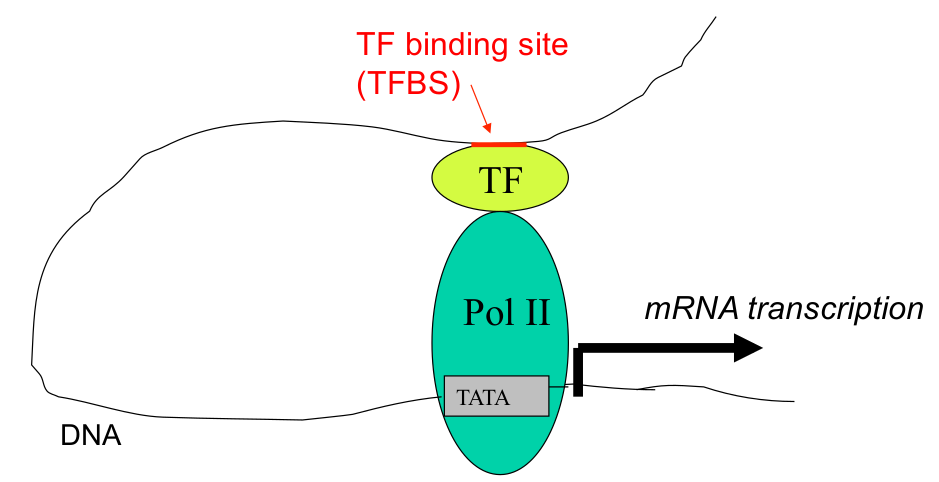
\includegraphics[width=\textwidth]{transcription}
\caption{Transcription regulation}
\label{Transcritpion regulation}
\end{figure}

\subsubsection{Bacterial transcription initiation}

RNA polymerase binds to the promoter region, which initiates transcription 
through interaction with transcription factors binding at different sites. 
It involves: Transcription Start Site (TSS), Open Reading Frame (ORF), 
Polymerase (Pol), Transcription Factor (TF), Transcription Factor Binding Site 
(TFBS).

\begin{figure}
\centering
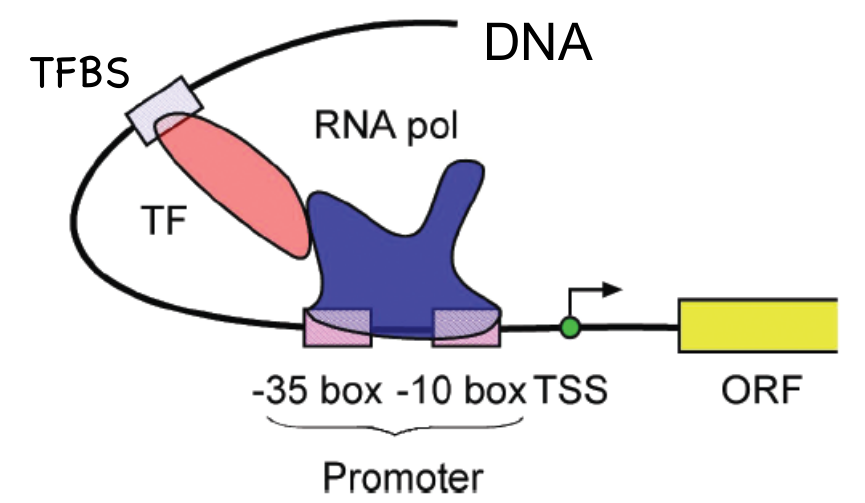
\includegraphics[width=\textwidth]{transcription_initiation_bacteria}
\caption{Schematic representation of elements involved in bacterial transcription initiation.}
\label{Transcritpion initiation in bacteria}
\end{figure}

\subsubsection{Eukaryotic transcription initiation}

Involves: Initiator sequence (Inr), ORF, Pol, TF, TFBS (there can be more than one).

\begin{figure}
\centering
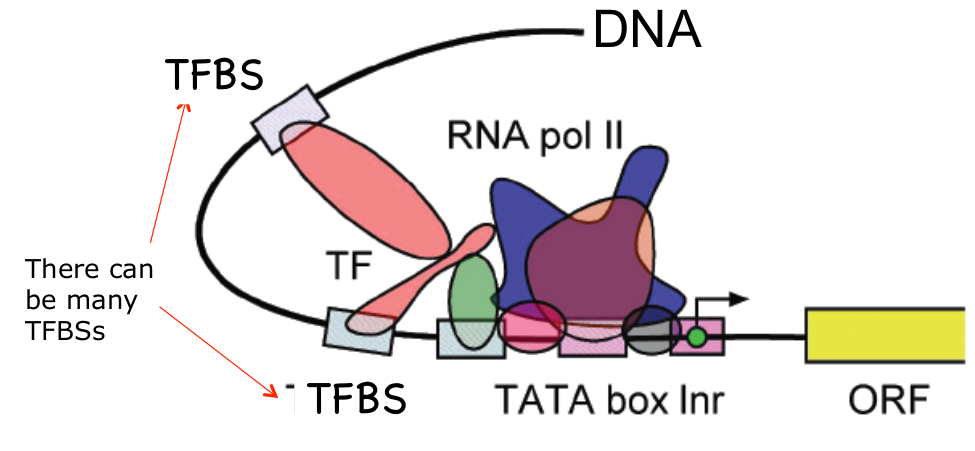
\includegraphics[width=\textwidth]{transcription_initiation_eukaryotic}
\caption{Schematic diagram of an eukaryotic promoter with transcription factors and RNA polymerase bound to the promoter.}
\label{Transcritpion initiation in eukaryotes}
\end{figure}

\subsection{Transcriptional regulation}

Gene expression is controlled by proximal and distal regulatory elements, 
commonly bound by combinatorial Transcription Factor (TF) complexes.

\begin{figure}
\centering
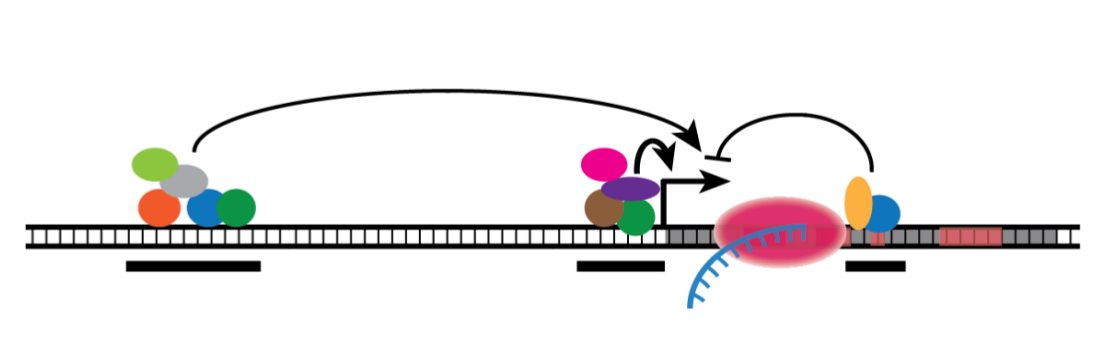
\includegraphics[width=\textwidth]{transcriptional_regulation}
\caption{Example fo transcriptional regulation that involves a promoter, exons 
and introns, TFs as regulatory elements.}
\label{Transcritpion initiation in eukaryotes}
\end{figure}

\subsubsection{Gene regulatory network}

Gene regulatory network models can be constructed from the TFs and the 
cis-regulatory elements with which they interact.

\subsubsection{Gene transcription}

\begin{enumerate}
\item Transcription factors (TF) are essential for transcription initialisation;
\item TFs bind to DNA-motifs called TF binding sites (TFBS);
\item Transcription is done by polymerase type II (eukaryotes);
\item mRNA must then move from nucleus to ribosomes (extranuclear) for translation;
\item In eukaryotes there can be many TF-binding sites upstream of an ORF 
(Open Reading Frame) which together regulate transcription;
\item TF binding sites can also be in other places (e.g. within gene regions, 
normally repressing transcription);
\item Transcription factors can activate (enhancers) or inhibit
(repressors) the transcription process.
\end{enumerate}

\subsubsection{DNA is packaged and protected}

DNA winds around histone proteins, forming a nucleosomes. Other proteins wind DNA
into more tightly packed form, the chromosome. Unwinding portions of the 
chromosome is important for mitosis, replication and making RNA.

\subsection{Translation: from mRNA to protein}

Translation from 4 nucleotides in (DNA and) RNA to 20 different amino acids in 
proteins. Translation uses codons (i.e. groups of three nucleotides); this gives 
$4^3$ = 64 possibilities. The 64 codons encode 20 amino acid types, a start codon
and stop codons. The encoding is given by a so-called codon table, linking each 
possible codon to its translated product. The codon table is redundant - i.e. 
different codons can encode the same amino acid. 

Translation involves mRNA (template), tRNA (amino acid carrier) and ribosome 
(poly-peptide generating enzyme).

\begin{figure}
\centering
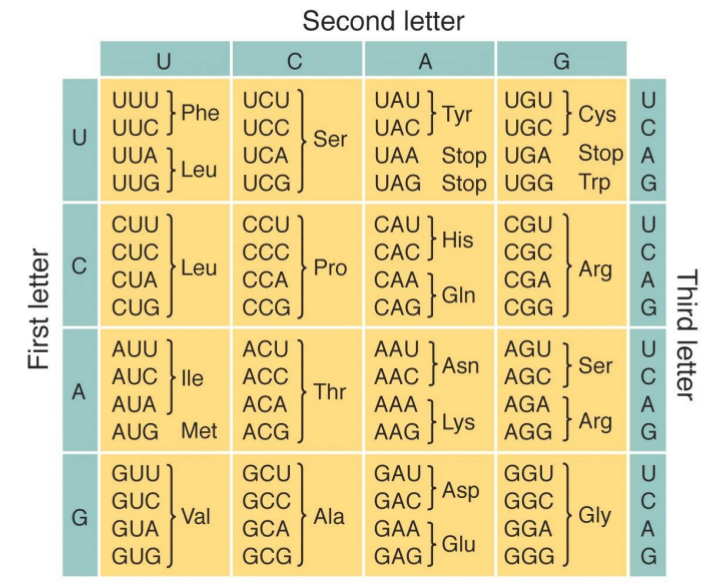
\includegraphics[width=\textwidth]{codon_table}
\caption{Codon table.}
\label{Codon table}
\end{figure}

\section{Evolution}

\subsection{DNA as an information carrier}

DNA has many good characteristichs to be an information carrier

\begin{itemize}
\item Stable at room temperature: DNA can last for hundreds of thousands of 
years;
\item Efficient: theoretical limit, store 1 zettabyte (1 billion TB) in 3-4
grams of DNA;
\item Usable: Next-Generation Sequencing (NGS) and analysis techniques bring 
reading and using the information artificially within reach.
\end{itemize}

\subsection{Divergent evolution}

There are four requirements for divergent evolution:

\begin{itemize}
\item Template structure providing stability (DNA);
\item Copying mechanism (meiosis);
\item Mechanism providing variation (mutations, insertions and deletions, 
crossing-over, etc.);
\item Selection: some traits lead to greater fitness of one individual 
relative to another. Darwin coined "survival of the fittest".
\end{itemize}

Evolution is a conservative process: the vast majority of mutations will not 
be selected (i.e. will not make it as they lead to worse performance or are 
even lethal) - this is called negative (or purifying or Darwinian) selection.

\subsection{Elements of evolution}

By repeated selection, evolution works as an optimisation process. However: 
the objective function that is optimised changes all the time (what is the 
fittest?), it is often a (spatially) local process, so it is a spatio-temporal 
locally (de)coupled process.

In the 1970s and early 80s, evolution became strongly viewed as an optimisation 
process (`optimal foraging', `optimal mating', etc.) - sometimes with amusing
consequences (e.g. optimality, non-optimality, pluralism, selection, drift).
The idea of overriding importance of selection became changed by the work of 
Motoo Kimura. His neutral selection theory was published in 1980.

\section{Homology/Orthology/Paralogy}

Two genes are hologous if they have a common evolutionary origin (a common 
ancestor). Orthologous genes are homologous (corresponding) genes in different 
species. Paralogous genes are homologous genes resulting from a duplication 
event within the same species (genome).

\subsection{Paralogy}

After a gene duplication event, paralogous sequences typically accumulate many 
mutations as a result of lowered selection pressure. Subfunctionalisation 
("splitting the old task") and Neofunctionalisation ("something new").

\begin{figure}
\centering
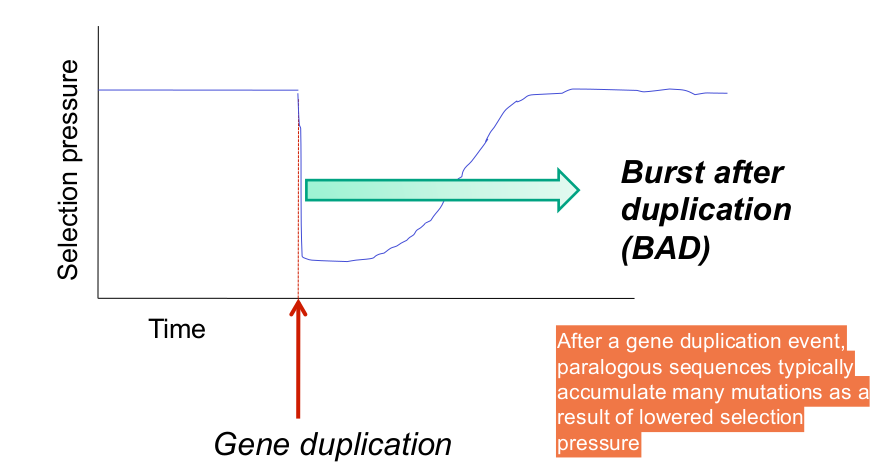
\includegraphics[width=\textwidth]{paralogy}
\caption{Selection pressure after a gene duplication}
\label{Paralogy}
\end{figure}

\subsection{Horizontal gene transfer}

Also referred to as lateral gene transfer or xenology. It is a non-hereditary 
exchange of DNA (horizontal versus vertical) that happens in bacteria. 
It leads to DNA regions that share no homology with evolutionary relatives, which
often complicates evolutionary analyses.

\subsection{Changing molecular sequences: DNA}

Mutations: changing nucleotides (`letters') within DNA, also called `point
mutations'. A and G are called purines, while C and T/U are called pyrimidine.
There are two possible modifications: transition and transversion.

\begin{figure}
\centering
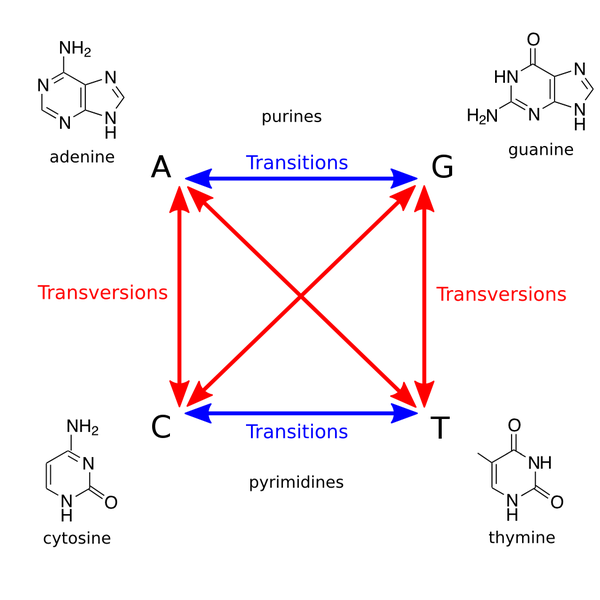
\includegraphics[width=\textwidth]{transition_transversion}
\caption{Differences between transition and transversion}
\label{Transition and Transversion}
\end{figure}

\subsubsection{Types of point mutations}

\begin{itemize}
\item Synonymous mutation: DNA mutation that does not lead to an amino acid
(protein) change;
\item Non-synonymous mutation: DNA mutation that does lead to an amino acid 
change
\begin{itemize}
\item Missense mutation: one amino acid replaced by another amino acid;
\item Nonsense mutation: amino acid replaced by stop codon (what happens with 
the protein?)
\end{itemize}
\end{itemize}

\subsection{Searching for similarities}

What is the function of the new gene?

The “lazy” investigation (i.e., no biological experiments, just bioinformatics 
techniques):

\begin{enumerate}
\item Find one or more protein sequences (in other species) that are similar to 
the unknown sequence;
\item Identify similarities and differences;
\item If sequences show enough similarity, we can assume they are homologous.
\end{enumerate}

\subsubsection{Homology principle}

Homology (common ancestry) makes it more likely that genes share the same 
structure and function.
When (an unknown) gene $X$ is homologous to (a known) gene $G$ it means that we 
gain a lot of information on $X$: what we know about $G$ can be transferred to $X$ 
as a good suggestion.

\subsubsection{Homology searching}

It starts with unknown query sequence. Thus, it searches for any putatively 
homologous sequence with annotation (i.e. with functional information). 
If found, transfer the information to the unknown sequence.